

\tikzset{every picture/.style={line width=0.75pt}} %set default line width to 0.75pt        

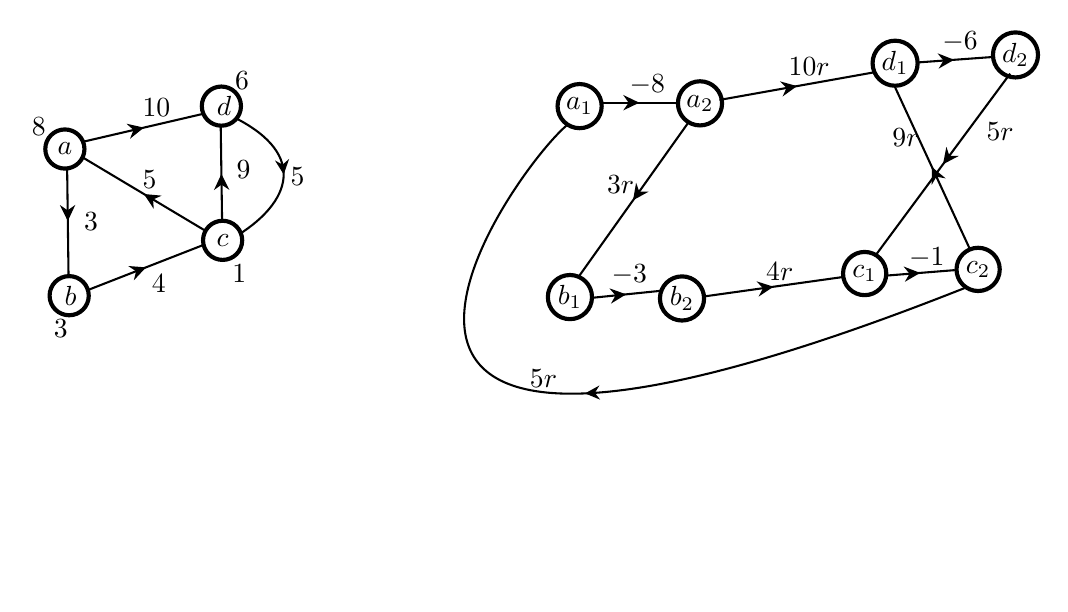
\begin{tikzpicture}[x=0.5pt,y=0.5pt,yscale=-1,xscale=1]
%uncomment if require: \path (0,288); %set diagram left start at 0, and has height of 288

%Straight Lines [id:da15240395104529547] 
\draw [color={rgb, 255:red, 0; green, 0; blue, 0 }  ,draw opacity=1 ][line width=0.75]    (51,102) -- (138,154) ;
\draw [shift={(94.5,128)}, rotate = 30.87] [fill={rgb, 255:red, 0; green, 0; blue, 0 }  ,fill opacity=1 ][line width=0.08]  [draw opacity=0] (11.61,-5.58) -- (0,0) -- (11.61,5.58) -- (7.71,0) -- cycle    ;
%Straight Lines [id:da35482909520855144] 
\draw [color={rgb, 255:red, 0; green, 0; blue, 0 }  ,draw opacity=1 ][line width=0.75]    (137,165) -- (55,197) ;
\draw [shift={(96,181)}, rotate = 158.68] [fill={rgb, 255:red, 0; green, 0; blue, 0 }  ,fill opacity=1 ][line width=0.08]  [draw opacity=0] (11.61,-5.58) -- (0,0) -- (11.61,5.58) -- (7.71,0) -- cycle    ;
%Straight Lines [id:da9934926023449607] 
\draw [color={rgb, 255:red, 0; green, 0; blue, 0 }  ,draw opacity=1 ][line width=0.75]    (39,109) -- (40,186) ;
\draw [shift={(39.5,147.5)}, rotate = 269.26] [fill={rgb, 255:red, 0; green, 0; blue, 0 }  ,fill opacity=1 ][line width=0.08]  [draw opacity=0] (11.61,-5.58) -- (0,0) -- (11.61,5.58) -- (7.71,0) -- cycle    ;
%Straight Lines [id:da7563500509285274] 
\draw [color={rgb, 255:red, 0; green, 0; blue, 0 }  ,draw opacity=1 ][line width=0.75]    (150,79) -- (151,148) ;
\draw [shift={(150.5,113.5)}, rotate = 89.17] [fill={rgb, 255:red, 0; green, 0; blue, 0 }  ,fill opacity=1 ][line width=0.08]  [draw opacity=0] (11.61,-5.58) -- (0,0) -- (11.61,5.58) -- (7.71,0) -- cycle    ;
%Straight Lines [id:da920349957299462] 
\draw [color={rgb, 255:red, 0; green, 0; blue, 0 }  ,draw opacity=1 ][line width=0.75]    (137.5,70) -- (51.5,90) ;
\draw [shift={(94.5,80)}, rotate = 166.91] [fill={rgb, 255:red, 0; green, 0; blue, 0 }  ,fill opacity=1 ][line width=0.08]  [draw opacity=0] (11.61,-5.58) -- (0,0) -- (11.61,5.58) -- (7.71,0) -- cycle    ;
%Curve Lines [id:da976908539012527] 
\draw    (160.5,73) .. controls (213.5,100) and (199.5,134) .. (163.5,157) ;
\draw [shift={(195.5,113.84)}, rotate = 263.76] [fill={rgb, 255:red, 0; green, 0; blue, 0 }  ][line width=0.08]  [draw opacity=0] (10.72,-5.15) -- (0,0) -- (10.72,5.15) -- (7.12,0) -- cycle    ;
%Straight Lines [id:da7434532828630788] 
\draw [color={rgb, 255:red, 0; green, 0; blue, 0 }  ,draw opacity=1 ][line width=0.75]    (479.5,62) -- (425.5,62) ;
\draw [shift={(452.5,62)}, rotate = 180] [fill={rgb, 255:red, 0; green, 0; blue, 0 }  ,fill opacity=1 ][line width=0.08]  [draw opacity=0] (11.61,-5.58) -- (0,0) -- (11.61,5.58) -- (7.71,0) -- cycle    ;
%Straight Lines [id:da3779476173807036] 
\draw [color={rgb, 255:red, 0; green, 0; blue, 0 }  ,draw opacity=1 ][line width=0.75]    (467.5,198) -- (418.5,203) ;
\draw [shift={(443,200.5)}, rotate = 174.17] [fill={rgb, 255:red, 0; green, 0; blue, 0 }  ,fill opacity=1 ][line width=0.08]  [draw opacity=0] (11.61,-5.58) -- (0,0) -- (11.61,5.58) -- (7.71,0) -- cycle    ;
%Straight Lines [id:da6132299382946279] 
\draw [color={rgb, 255:red, 0; green, 0; blue, 0 }  ,draw opacity=1 ][line width=0.75]    (680.5,183) -- (630.5,187) ;
\draw [shift={(655.5,185)}, rotate = 175.43] [fill={rgb, 255:red, 0; green, 0; blue, 0 }  ,fill opacity=1 ][line width=0.08]  [draw opacity=0] (11.61,-5.58) -- (0,0) -- (11.61,5.58) -- (7.71,0) -- cycle    ;
%Straight Lines [id:da8250679630157668] 
\draw [color={rgb, 255:red, 0; green, 0; blue, 0 }  ,draw opacity=1 ][line width=0.75]    (707.5,29) -- (652.5,33) ;
\draw [shift={(680,31)}, rotate = 175.84] [fill={rgb, 255:red, 0; green, 0; blue, 0 }  ,fill opacity=1 ][line width=0.08]  [draw opacity=0] (11.61,-5.58) -- (0,0) -- (11.61,5.58) -- (7.71,0) -- cycle    ;
%Straight Lines [id:da07369024589592021] 
\draw [color={rgb, 255:red, 0; green, 0; blue, 0 }  ,draw opacity=1 ][line width=0.75]    (408.5,188) -- (487.5,77) ;
\draw [shift={(448,132.5)}, rotate = 305.44] [fill={rgb, 255:red, 0; green, 0; blue, 0 }  ,fill opacity=1 ][line width=0.08]  [draw opacity=0] (11.61,-5.58) -- (0,0) -- (11.61,5.58) -- (7.71,0) -- cycle    ;
%Straight Lines [id:da320585315348929] 
\draw [color={rgb, 255:red, 0; green, 0; blue, 0 }  ,draw opacity=1 ][line width=0.75]    (599.5,188) -- (499.5,202) ;
\draw [shift={(549.5,195)}, rotate = 172.03] [fill={rgb, 255:red, 0; green, 0; blue, 0 }  ,fill opacity=1 ][line width=0.08]  [draw opacity=0] (11.61,-5.58) -- (0,0) -- (11.61,5.58) -- (7.71,0) -- cycle    ;
%Curve Lines [id:da28058077156757066] 
\draw    (687.5,196) .. controls (149.5,409) and (359.5,112) .. (400.5,78) ;
\draw [shift={(413.28,272.08)}, rotate = 356.86] [fill={rgb, 255:red, 0; green, 0; blue, 0 }  ][line width=0.08]  [draw opacity=0] (10.72,-5.15) -- (0,0) -- (10.72,5.15) -- (7.12,0) -- cycle    ;
%Straight Lines [id:da43509653737521126] 
\draw [color={rgb, 255:red, 0; green, 0; blue, 0 }  ,draw opacity=1 ][line width=0.75]    (636.5,49) -- (691.5,168) ;
\draw [shift={(664,108.5)}, rotate = 65.19] [fill={rgb, 255:red, 0; green, 0; blue, 0 }  ,fill opacity=1 ][line width=0.08]  [draw opacity=0] (11.61,-5.58) -- (0,0) -- (11.61,5.58) -- (7.71,0) -- cycle    ;
%Straight Lines [id:da6639766439417539] 
\draw [color={rgb, 255:red, 0; green, 0; blue, 0 }  ,draw opacity=1 ][line width=0.75]    (623.5,172) -- (720.5,41) ;
\draw [shift={(672,106.5)}, rotate = 306.52] [fill={rgb, 255:red, 0; green, 0; blue, 0 }  ,fill opacity=1 ][line width=0.08]  [draw opacity=0] (11.61,-5.58) -- (0,0) -- (11.61,5.58) -- (7.71,0) -- cycle    ;
%Straight Lines [id:da10266580678651627] 
\draw [color={rgb, 255:red, 0; green, 0; blue, 0 }  ,draw opacity=1 ][line width=0.75]    (622.5,40) -- (510.5,60) ;
\draw [shift={(566.5,50)}, rotate = 169.88] [fill={rgb, 255:red, 0; green, 0; blue, 0 }  ,fill opacity=1 ][line width=0.08]  [draw opacity=0] (11.61,-5.58) -- (0,0) -- (11.61,5.58) -- (7.71,0) -- cycle    ;

% Text Node
\draw (91.24,108.53) node [anchor=north west][inner sep=0.75pt]   [align=left] {$\displaystyle 5$};
% Text Node
\draw  [line width=1.5]   (37.38, 95.47) circle [x radius= 14.15, y radius= 14.15]   ;
\draw (37.38,95.47) node   [align=left] {$\displaystyle a$};
% Text Node
\draw  [line width=1.5]   (40.48, 201.47) circle [x radius= 14.15, y radius= 14.15]   ;
\draw (34.98,201.47) node [anchor=west] [inner sep=0.75pt]   [align=left] {$\displaystyle b$};
% Text Node
\draw  [line width=1.5]   (151.38, 161.47) circle [x radius= 14.15, y radius= 14.15]   ;
\draw (151.38,161.47) node   [align=left] {$\displaystyle c$};
% Text Node
\draw (98,184) node [anchor=north west][inner sep=0.75pt]   [align=left] {$\displaystyle 4$};
% Text Node
\draw (49,139.47) node [anchor=north west][inner sep=0.75pt]   [align=left] {$\displaystyle 3$};
% Text Node
\draw  [line width=1.5]   (150.48, 64.47) circle [x radius= 14.15, y radius= 14.15]   ;
\draw (144.98,64.47) node [anchor=west] [inner sep=0.75pt]   [align=left] {$\displaystyle d$};
% Text Node
\draw (159.24,101.53) node [anchor=north west][inner sep=0.75pt]   [align=left] {$\displaystyle 9$};
% Text Node
\draw (91.24,56.53) node [anchor=north west][inner sep=0.75pt]   [align=left] {$\displaystyle 10$};
% Text Node
\draw (11.24,70.53) node [anchor=north west][inner sep=0.75pt]   [align=left] {$\displaystyle 8$};
% Text Node
\draw (27.24,216.53) node [anchor=north west][inner sep=0.75pt]   [align=left] {$\displaystyle 3$};
% Text Node
\draw (156.24,176.53) node [anchor=north west][inner sep=0.75pt]   [align=left] {$\displaystyle 1$};
% Text Node
\draw (158.24,37.53) node [anchor=north west][inner sep=0.75pt]   [align=left] {$\displaystyle 6$};
% Text Node
\draw (198.24,106.53) node [anchor=north west][inner sep=0.75pt]   [align=left] {$\displaystyle 5$};
% Text Node
\draw  [line width=1.5]   (409.38, 64.47) circle [x radius= 15.95, y radius= 15.95]   ;
\draw (409.38,64.47) node   [align=left] {$\displaystyle a_{1}$};
% Text Node
\draw  [line width=1.5]   (496.38, 62.47) circle [x radius= 15.95, y radius= 15.95]   ;
\draw (496.38,62.47) node   [align=left] {$\displaystyle a_{2}$};
% Text Node
\draw  [line width=1.5]   (402.38, 202.47) circle [x radius= 15.95, y radius= 15.95]   ;
\draw (402.38,202.47) node   [align=left] {$\displaystyle b_{1}$};
% Text Node
\draw  [line width=1.5]   (483.38, 203.47) circle [x radius= 15.95, y radius= 15.95]   ;
\draw (483.38,203.47) node   [align=left] {$\displaystyle b_{2}$};
% Text Node
\draw  [line width=1.5]   (615.38, 185.47) circle [x radius= 15.62, y radius= 15.62]   ;
\draw (615.38,185.47) node   [align=left] {$\displaystyle c_{1}$};
% Text Node
\draw  [line width=1.5]   (697.38, 182.47) circle [x radius= 15.62, y radius= 15.62]   ;
\draw (697.38,182.47) node   [align=left] {$\displaystyle c_{2}$};
% Text Node
\draw  [line width=1.5]   (637.38, 33.47) circle [x radius= 16.28, y radius= 16.28]   ;
\draw (637.38,33.47) node   [align=left] {$\displaystyle d_{1}$};
% Text Node
\draw  [line width=1.5]   (724.38, 27.47) circle [x radius= 16.28, y radius= 16.28]   ;
\draw (724.38,27.47) node   [align=left] {$\displaystyle d_{2}$};
% Text Node
\draw (443.24,39.53) node [anchor=north west][inner sep=0.75pt]   [align=left] {$\displaystyle -8$};
% Text Node
\draw (430.24,176.53) node [anchor=north west][inner sep=0.75pt]   [align=left] {$\displaystyle -3$};
% Text Node
\draw (645.24,164.53) node [anchor=north west][inner sep=0.75pt]   [align=left] {$\displaystyle -1$};
% Text Node
\draw (669.24,8.53) node [anchor=north west][inner sep=0.75pt]   [align=left] {$\displaystyle -6$};
% Text Node
\draw (558.24,27.53) node [anchor=north west][inner sep=0.75pt]   [align=left] {$\displaystyle 10r$};
% Text Node
\draw (371.24,252.53) node [anchor=north west][inner sep=0.75pt]   [align=left] {$\displaystyle 5r$};
% Text Node
\draw (427,112.47) node [anchor=north west][inner sep=0.75pt]   [align=left] {$\displaystyle 3r$};
% Text Node
\draw (542,175) node [anchor=north west][inner sep=0.75pt]   [align=left] {$\displaystyle 4r$};
% Text Node
\draw (633.24,78.53) node [anchor=north west][inner sep=0.75pt]   [align=left] {$\displaystyle 9r$};
% Text Node
\draw (701.24,74.53) node [anchor=north west][inner sep=0.75pt]   [align=left] {$\displaystyle 5r$};


\end{tikzpicture}

